\documentclass{report}
\usepackage{graphicx}
\usepackage{wasysym}
\usepackage{listings}
\usepackage{color}
\usepackage{multirow}
\usepackage{arydshln}
\usepackage{csvsimple}
\usepackage{pgfplotstable}
\usepackage{booktabs,colortbl}
\usepackage{subfigure}
\usepackage{caption}
\usepackage{lscape}
\usepackage{geometry}
\usepackage{algorithm2e}
\usepackage{natbib}
\usepackage{amsmath}

\graphicspath{{test_results/}}

\newcommand*\cbox{\item[\XBox]}
\newcommand*\uncbox{\item[\Square]}

\newcommand{\tempsfolder}{../KDeepBeliefNetwork_summer/test_results}

\definecolor{dkgreen}{rgb}{0,0.6,0}
\definecolor{gray}{rgb}{0.5,0.5,0.5}
\definecolor{mauve}{rgb}{0.58,0,0.82}

\lstset{frame=tb,
  language=Python,
  aboveskip=3mm,
  belowskip=3mm,
  showstringspaces=false,
  columns=flexible,
  basicstyle={\small\ttfamily},
  numbers=none,
  numberstyle=\tiny\color{gray},
  keywordstyle=\color{blue},
  commentstyle=\color{dkgreen},
  stringstyle=\color{mauve},
  breaklines=true,
  breakatwhitespace=true,
  tabsize=3
}


\begin{document}

%\chapter*{\LARGE{Discriminative and Generative DBN: Digits}}
\section{Background}
\subsection{Energy-based models}
Energy-based models discover dependencies between variables by assigning a scalar energy to each configuration of the variables. Inference is done by finding configurations of desired unobserved variables for which the energy is minimized. Learning consists in adjusting the energy function until the observed configurations are assigned lower energies than the unobserved ones \cite{LeCun}. The probability distribution of the variables is defined though an energy function such that
\begin{equation}
p(v) = \frac{e^{-E(v)}}{Z}
\end{equation}
where $Z$ is the partition function, a normalizing constant, and $E(x)$ is the energy function given $v$.

\subsection{Restricted Boltzmann Machines}

A Restricted Boltzmann machine (RBM) is a two-layer network that models the probability distribution over a vector of visible variables $v$ and a vector of latent, or hidden, variables $h$, using symmetrically weighted connections\cite{Mnih}. Here, the values of the binary input vector are the visible units, while the feature detectors are the hidden units. The probability distribution $p(v,h)$ is given by:
\begin{equation}
p(v,h) = \frac{e^{-E(v,h)}}{Z}
\end{equation}

where the energy function of an RBM is defined as:
\begin{equation}
E(v, h) = -vWh - vb - hc
\end{equation}

$W$ is the matrix of the weights connecting visible units $v_i$ to hidden units $h_j$, and $b$, $c$ are the biases of the visible and hidden layers, respectively. $p(v)$ is obtained by marginalizing out $h$ from the joint distribution, and we get:

\begin{align}
p(v) &=  \sum_h \frac{e^{-E(v,h)}}{Z} \nonumber \\
& = \frac{e^{-\mathcal{F}(v)}}{Z}
\end{align}

where $\mathcal{F}(v)$ is the free energy formula:

\begin{align}
\mathcal{F}(v) & = -\log \sum_h e^{-E(v,h)} \nonumber \\
& = -vb - \sum_j \log (1 + e^{c_j + W_j v})
\label{eq:fev}
\end{align}


\subsection{DBNs: Stacking RBMs for Classification}
RBMs have been used both as discriminative and generative models, and when stacked, the output of the hidden layers turns into input for the next hidden layers, creating 'feature feature-detectors.' Stacked RBMs have mostly been used as learning modules to form Deep Belief Networks (DBNs) \cite{Hinton} \cite{Schmah}. A DBN is a graphical model that learns to extract deep hierarchical representations from data as its structure consists of undirected connections at the top hidden layer, and directed connections in the lower layers \cite{Ngiam}. There can be as many hidden layers as desired, and together they compose a single, multilayer model.

As a classifier, the model is discriminatively trained by stochastic gradient descent to model the joint distribution of $v$ and target class $y$, a 'softmax' label unit with a 'one out of C' representation. A separate RBM is trained for each class, and classification is determined by the free energy ($\mathcal{F}$) of each network \cite{Elfwing}. The free energy equation of a discriminative model becomes \cite{Louradour}:

\begin{align}
\mathcal{F}(v, y) & = -\log \sum_h e^{-E(v,h,y)} \nunumber \\
& = -yd - \sum_j \log (1 + e^{c_j + W_j v + U_j y})
\label{eq:fevy}
\end{align}

where $d$ is the bias of class label $y$, and $U$ the class weight matrix. 


\subsection{DBNs: Stacking RBMs for Prediction}
Stacked RBMs have also been used with non-binary categories and continuous-valued inputs, and applied to tasks such as speech synthesis \cite{Jaitly}, fMRI image classification \cite{Schmah}, and time series forecasting \cite{Ginzburg} \cite{Kuremoto}. Continous-valued input $x$ is reconstructed to expected input $v$, and the output of the last feature-detecting RBM unit is the coarse prediction $\hat{x}$. Training consists in fine-tuning the model by adjusting the weights based on the value of $\mathcal{F}$ until the obtention of a refined prediction determined by the error rate of $\hat{x}$ compared to $x$\cite{Kuremoto}. The free energy equation for continuous, Gaussian-distributed visible units becomes \cite{Schmah}:

\begin{align}
\mathcal{F}(v) & = -\log \sum_h e^{-E(v,h)} \nonumber \\
& =  - \sum_j \log (1 + e^{c_j + W_j v}) + \frac{1}{2} \sum_i (v - b)^2
\label{eq:fegbv}
\end{align}




\section{Experiment: The MNIST dataset}
The data used for the evaluation of the classification task is the MNIST dataset, a collection of handwritten digits represented in vectors of strongly bimodal input values. In the original dataset, each pixel of the image is represented by a value between 0 and 255, where 0 is black, 255 is white and values in between are different shades of gray.


To test the classifier for performance when dealing with possibly erroneous data, we added noise to the input data. The input data are vectors of 784 values normalized to floats between 0 and 1, each corresponding to a pixel of a 28x28 digital representation of a handwritten digit, where 0 is black, and 1 is white.

% example of corruption
\begin{figure}[h!]
	\subfigure[No corruption]{
	\includegraphics[width=.28\textwidth]{five_img}}
	\subfigure[$pc$=4 and $l$=1]{
	\includegraphics[width=.28\textwidth]{corr_five_image}}
	\subfigure[$pc$=4 and $l$=5]{
	\includegraphics[width=.28\textwidth]{corr_five_c5_image}}
	\caption{An example of an inverted digitalized handwritten 5 and the result after the two types of corruption processes.}
\end{figure}

\subsection{Digit classification}


\textbf{check the layer configuration}
The DBN consists of three RBMs, where the first is a Bernouilli RBM, and the deeper layers binary RBMs. \textbf{check}. The model was trained with a configuration of 500 $\leftrightarrow$ 2000 $\leftrightarrow$ 2000. The test dataset contains 10000 image vectors. The error rates and $\mathcal{F}$ values are recorded for the control set, where the $\mathcal{F}$ of the whole network is calculated by adding the $\mathcal{F}(v,y)$ (eq.~\eqref{eq:fevy}) of the top class RBM, to the $\mathcal{F}(v)$ (eq.~\eqref{eq:fev}) of the other RBMs.

For the simulated noised dataset, each individual image vector of the test set is subject to random corruption (where values are replaced with 1's), determined by a noise percentage $pc$ and length $l$. The corruption percentage is between 0 and 15\%, and the length is between 1 and 5 (pixels). Table~\ref{table:control} shows the $\mathcal{F}$ mean for each set, and the classification error rate as the corruption percentage is incremented. The classification confusion matrices are presented in Figure~\ref{fig:CM}.


There are many techniques to discover if data is reliable, such as clustering for outlier detection cite{}, or training models with noise for robustness as in denoising autoencoders \cite{Vincent}, but we chose to inspect a measure that is specific to EBMs. We analyzed the behaviour of $\mathcal{F}$ outside of its role in the training of the model. In training, the energy determines the probability of a joint configuration of the visible and hidden units, and is used in the definition of the model's learning. In testing, energy can be used as a marker for unexpected input data since it is directly affected by the values of the visible layer. Figure~\ref{fig:nrgs} shows that, as expected, $\mathcal{F}$ evolves proportionally to the amount of added noise. 

% control set table
\begin{table}
	\begin{center}
		\pgfplotstabletypeset[
			col sep=comma,
			string type,
			every head row/.style={before row=\hline,
				after row=\hline
			},
			every last row/.style={after row=\hline},
			columns/pc/.style={column name={\% corruption}, column type={|c}},
			columns/Fmean/.style={column name={mean $\mathcal{F}$}, column type={|r}},
			columns/er/.style={column name={error rate}, column type={|c|}},
			]{test_results/errfe_stats_0n.csv}
	\end{center}
	\caption{mean of $\mathcal{F}$ and classification error rate as noise is increased}
	\label{table:control}
\end{table}

% confusion matrices
\begin{figure}
\begin{center}
	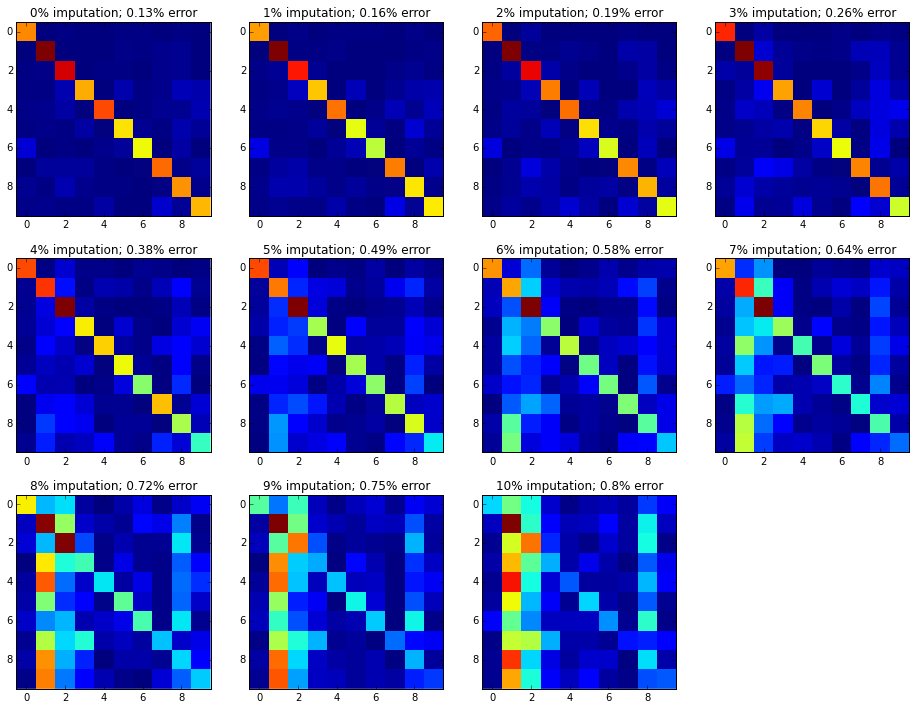
\includegraphics[width=\textwidth]{confusion_matrices}
	\caption{Classification confusion matrices for control dataset}
	\label{fig:CM}
\end{center}
\end{figure}

% FE boxplots
\begin{figure}
	\centering
		\includegraphics[width=.7\textwidth]{FE_boxplots0n1c}
	\caption{Free energies of each input vector as noise is increased}
	\label{fig:nrgs}
\end{figure}


From the energy formula, we can see how $\mathcal{F}$ is directly affected. A deviation from an expected $v$ will be captured when sent through the network as it will be affected according to the model's learned weights. This deviation will raise $\mathcal{F}$ and act as a flag for an undesirable configuration, or in our case, noisy data.


\subsection{Reconstruction}
In an attempt to fix the noisy data, we look to the generative powers of the network to reconstruct the corrupted vector. As a generator, the bottom-up pass is the initialization process, or 'wake' phase, and the top-down, or 'sleep' phase, is the generation process. This is different from denoising autoencoders in many ways. First, the model is not trained with noise, so the model attempts reconstruction at time of use, when encountering noise for the first time. Then, the reconstruction is not done by maximizing a variational bound, as proposed by \citet{Vincent}, but simply from a top-down generation process when triggered by a threshold, again, outside of training. Finally, the reconstruction is carried out given a class and the learned weights, and generates a new, possibly different form of the digit. \citet{Vincent}'s reconstruction is realized through a deterministic mapped representation of a corrupted $v$, and learned weights.

The issue here is that for the generation task, the model must be provided a class of the desired digit. Our class prediction $y$ is unreliable, as seen from the increasing error rates, and the wrong class will generate the wrong digit. We therefore must choose a threshold to alert us when a predicted class cannot be trusted.
% One important difference is that deterministic autoencoders consider that real valued mean as their hidden representation whereas stochastic RBMs sample a binary hidden representation from that mean. 


$\mathcal{F}$ is measured using arbitrary units, and its range is specific to each model. The threshold must therefore be chosen based on individual models. The maximum recorded value of $\mathcal{F}$ from the control set was chosen as the threshold for our classifier. During the wake phase, if the calculated $\mathcal{F}$ of a given input vector is greater than the set threshold, it is sent back to the first layer and is run through the wake phase $n$ times. The prediction of each reclassification is stored and the class with the greatest count is then chosen as the class label to be clamped in the sleep phase. This new image is weighted, fused with the original one that has also been weighted, and reclassified for evaluation. The results are presented in Table~\ref{table:results}. Algorithm ~\ref{alg:mnist} demonstrates how the reclassification process is carried out, and an example of mixing the process is demonstrated in Figure~\ref{fig:mixing}.

\smallskip

\begin{algorithm}[H]
	\KwData{digit image vector}
	\KwResult{digit class}
 	corrupt $pc$\% of input vector with length $l$\;
	classify $x_{corr}$\;
	calculate $\mathcal{F}$ of network\;
	\eIf{$\mathcal{F} > threshold$}{
		reclassify $n$ times\;
		class with most count becomes current class\;
		generate with clamped class label\;
		mix weighted $x_{corr}$ and weighted $x_{gen}$\;	
		classify $x_{gen}$\;
		}{
	return class of $x_{gen}$\;
	}
	\caption{Reclassification and Generation}
	\label{alg:mnist}
\end{algorithm}

\smallskip

%result tables
{\newgeometry{left=1.6cm, right=1.6cm, top=2cm}
\begin{table}
\footnotesize
\centering
	\subtable[pc=0, c=1]{
		\pgfplotstabletypeset[
			col sep=comma,
			string type,
			every head row/.style={%
				before row={\cline{3-6}
					\multicolumn{2}{c|}{ } & \multicolumn{2}{c||}{Reconstruction} & \multicolumn{2}{c|}{Reclassification}\\
				\hline},
				after row=\hline
			},
			every first row/.style={
				before row={\rowcolor[gray]{0.9}
				\hline},
				after row=\hline,
			},
			every last row/.style={after row=\hline},
			columns/pc/.style={column name=noise \%, column type={|c}},
			columns/n/.style={column name=n, column type={|r}},
			columns/{FE rr}/.style={column name={mean $\mathcal{F}$}, column type={|c}},
			columns/{err rr}/.style={column name={error rate}, column type={|c|}},
			columns/{FE r}/.style={column name={mean $\mathcal{F}$}, column type={|c}},
			columns/{err r}/.style={column name={error rate}, column type={|c|}},
			]{test_results/errfe_stats0c.csv}}
			\\
	\subtable[c=1]{
		\pgfplotstabletypeset[
			col sep=comma,
			string type,
			every head row/.style={%
				before row={\cline{3-6}
					\multicolumn{2}{c|}{ } & \multicolumn{2}{c||}{Reconstruction} & \multicolumn{2}{c|}{Reclassification}\\
				\hline},
				after row=\hline
			},
			every first row/.style={
				before row={\rowcolor[gray]{0.9}
				},
				after row=\hline},
			every nth row={5}{%
				before row={\hline
				\rowcolor[gray]{0.9}
				},
				after row=\hline,
			},
			every last row/.style={after row=\hline},
			columns/pc/.style={column name=noise \%, column type={|c}},
			columns/n/.style={column name=n, column type={|r}},
			columns/{FE rr}/.style={column name={mean $\mathcal{F}$}, column type={|c}},
			columns/{err rr}/.style={column name={error rate}, column type={|c|}},
			columns/{FE r}/.style={column name={mean $\mathcal{F}$}, column type={|c}},
			columns/{err r}/.style={column name={error rate}, column type={|c|}},
			]{test_results/errfe_stats1c.csv}
	}
	\subtable[c=2]{
		\pgfplotstabletypeset[
			col sep=comma,
			string type,
			every head row/.style={%
				before row={\cline{3-6}
					\multicolumn{2}{c|}{ } & \multicolumn{2}{c||}{Reconstruction} & \multicolumn{2}{c|}{Reclassification}\\
				\hline},
				after row=\hline
			},
			every first row/.style={
				before row={\rowcolor[gray]{0.9}
				},
				after row=\hline},
			every nth row={5}{%
				before row={\hline
				\rowcolor[gray]{0.9}
				},
				after row=\hline,
			},
			every last row/.style={after row=\hline},
			columns/pc/.style={column name=noise \%, column type={|c}},
			columns/n/.style={column name=n, column type={|r}},
			columns/{FE rr}/.style={column name={mean $\mathcal{F}$}, column type={|c}},
			columns/{err rr}/.style={column name={error rate}, column type={|c|}},
			columns/{FE r}/.style={column name={mean $\mathcal{F}$}, column type={|c}},
			columns/{err r}/.style={column name={error rate}, column type={|c|}},
			]{test_results/errfe_stats2c.csv}
	}
	\subtable[c=5]{
		\pgfplotstabletypeset[
			col sep=comma,
			string type,
			every head row/.style={%
				before row={\cline{3-6}
					\multicolumn{2}{c|}{ } & \multicolumn{2}{c||}{Reconstruction} & \multicolumn{2}{c|}{Reclassification}\\
				\hline},
				after row=\hline
			},
			every first row/.style={
				before row={\rowcolor[gray]{0.9}
				},
				after row=\hline},
			every nth row={5}{%
				before row={\hline
				\rowcolor[gray]{0.9}
				},
				after row=\hline,
			},
			every last row/.style={after row=\hline},
			columns/pc/.style={column name=noise \%, column type={|c}},
			columns/n/.style={column name=n, column type={|r}},
			columns/{FE rr}/.style={column name={mean $\mathcal{F}$}, column type={|c}},
			columns/{err rr}/.style={column name={error rate}, column type={|c|}},
			columns/{FE r}/.style={column name={mean $\mathcal{F}$}, column type={|c}},
			columns/{err r}/.style={column name={error rate}, column type={|c|}},
			]{test_results/errfe_stats5c.csv}
	}
	\subtable[c=10]{
		\pgfplotstabletypeset[
			col sep=comma,
			string type,
			every head row/.style={%
				before row={\cline{3-6}
					\multicolumn{2}{c|}{ } & \multicolumn{2}{c||}{Reconstruction} & \multicolumn{2}{c|}{Reclassification}\\
				\hline},
				after row=\hline
			},
			every first row/.style={
				before row={\rowcolor[gray]{0.9}
				},
				after row=\hline},
			every nth row={5}{%
				before row={\hline
				\rowcolor[gray]{0.9}
				},
				after row=\hline,
			},
			every last row/.style={after row=\hline},
			columns/pc/.style={column name=noise \%, column type={|c}},
			columns/n/.style={column name=n, column type={|r}},
			columns/{FE rr}/.style={column name={mean $\mathcal{F}$}, column type={|c}},
			columns/{err rr}/.style={column name={error rate}, column type={|c|}},
			columns/{FE r}/.style={column name={mean $\mathcal{F}$}, column type={|c}},
			columns/{err r}/.style={column name={error rate}, column type={|c|}},
			]{test_results/errfe_stats10c.csv}
	}
	\caption{Reconstruction vs. Reclassification alone: Mean of $\mathcal{F}$ and error rates by percentage of corruption and reclassification iterations. (a) are the results for the control set. (b)-(e) are the results for the corrupted set, by length of corruption.}
	\label{table:results}
\end{table}
}

%3-bps graphs
{\newgeometry{top=.7cm}
\begin{figure}
	\centering
	\subfigure[c=1]{
		\includegraphics[width=\textwidth]{PFE_boxplots50n1c}
	}
	\subfigure[c=2]{
		\includegraphics[width=\textwidth]{PFE_boxplots50n2c}
	}
	\subfigure[c=5]{
		\includegraphics[width=\textwidth]{PFE_boxplots50n5c}
	}
	\subfigure[c=10]{
		\includegraphics[width=\textwidth]{PFE_boxplots50n10c}
	}
	\caption{$\mathcal{F}$ measures for control set, reconstruction set, and reclassification alone set at $n$ = 50. -252.38 is the highest recorded $\mathcal{F}$ at 0\% corruption, and is set as threshold for unreliability.}
	\label{fig:FE_3bp}
\end{figure}
}

% error line graphs
{\newgeometry{left=1cm, top=.1cm, bottom=.1cm}
\begin{landscape}
\begin{figure}
	\centering
	\subfigure[n=25, c=1]{\includegraphics[width=0.35\textwidth]{Perr_linegraph25n1c}}
	\subfigure[n=25, c=2]{\includegraphics[width=0.35\textwidth]{Perr_linegraph25n2c}}
	\subfigure[n=25, c=5]{\includegraphics[width=0.35\textwidth]{Perr_linegraph25n5c}}
	\subfigure[n=25, c=10]{\includegraphics[width=0.35\textwidth]{Perr_linegraph25n10c}}
	\subfigure[n=50, c=1]{\includegraphics[width=0.35\textwidth]{Perr_linegraph50n1c}}
	\subfigure[n=50, c=2]{\includegraphics[width=0.35\textwidth]{Perr_linegraph50n2c}}
	\subfigure[n=50, c=5]{\includegraphics[width=0.35\textwidth]{Perr_linegraph50n5c}}
	\subfigure[n=50, c=10]{\includegraphics[width=0.35\textwidth]{Perr_linegraph50n10c}}
	\subfigure[n=100, c=1]{\includegraphics[width=0.35\textwidth]{Perr_linegraph100n1c}}
	\subfigure[n=100, c=2]{\includegraphics[width=0.35\textwidth]{Perr_linegraph100n2c}}
	\subfigure[n=100, c=5]{\includegraphics[width=0.35\textwidth]{Perr_linegraph100n5c}}
	\subfigure[n=100, c=10]{\includegraphics[width=0.35\textwidth]{Perr_linegraph100n10c}}
	\subfigure[n=1000, c=1]{\includegraphics[width=0.35\textwidth]{Perr_linegraph1000n1c}}
	\subfigure[n=1000, c=2]{\includegraphics[width=0.35\textwidth]{Perr_linegraph1000n2c}}
	\subfigure[n=1000, c=5]{\includegraphics[width=0.35\textwidth]{Perr_linegraph1000n5c}}
	\subfigure[n=1000, c=10]{\includegraphics[width=0.35\textwidth]{Perr_linegraph1000n10c}}
	\caption{Error rates: Control vs. Reconstruction vs. Reclassification alone for all $n$s and $c$s.}
	\label{fig:errgraph}
\end{figure}
\end{landscape}
}

\subsection{Analysis}
While running the reclassification and reconstruction trials, we saw that there was an important drop in error rates in the classification of the mixed images, but what's more is that reclassification alone was even more successful. The results table therefore also includes the reclassification without generation results.

From the graphs in Figure~\ref{fig:errgraph}, we can see that by simply averaging the $n$-reclassification output, the results in terms of error rate are the best. However, if the goal is to reconstruct the input data to rid it of noise, the added reconstruction is also successful, as seen by both the error rates and the values of $\mathcal{F}$. 

The number of reclassification iterations has an effect as well, as shown in Table~\ref{table:results}. The greater the $n$, the lower the error rates. The optimal number for reclassification iterations was set to $n$=50 and has been chosen based on the favourable results and the amount of time required to reclassify.

Table~\ref{table:results_c} shows the effect of the length of corruption. As it is increased, the error rate increases as well, but only until the 5\% corruption level. At 10\% corruption, the error rate decreases as the length increases, both for reconstruction and reclassification.

\textbf{why?}



% c result tables
\begin{table}
	\begin{footnotesize}
		\subtable[Reconstruction]{
			\pgfplotstabletypeset[
				col sep=comma,
				header=false,
				every head row/.style={%
					output empty row,
					before row={%
						\cline{2-16}
						& \multicolumn{3}{|c|}{1 \% corruption}%
						& \multicolumn{3}{c|}{2 \% corruption}%
						& \multicolumn{3}{c|}{5 \% corruption}%
						& \multicolumn{3}{c|}{10 \% corruption}%
						& \multicolumn{3}{c|}{15 \% corruption}\\
					},
					after row=\hline
				},
				every last row/.style={after row=\hline},
				display columns/0/.style={string type, column type={c|}}
		]{test_results/err_stats_c_rr.csv}
		}
		\subtable[Reclassification]{
			\pgfplotstabletypeset[
				col sep=comma,
				header=false,
				every head row/.style={%
					output empty row,
					before row={%
						\cline{2-16}
						& \multicolumn{3}{|c|}{1 \% corruption}%
						& \multicolumn{3}{c|}{2 \% corruption}%
						& \multicolumn{3}{c|}{5 \% corruption}%
						& \multicolumn{3}{c|}{10 \% corruption}%
						& \multicolumn{3}{c|}{15 \% corruption}\\
					},
					after row=\hline
				},
				every last row/.style={after row=\hline},
				display columns/0/.style={string type, column type={c|}},
		]{test_results/err_stats_c_r.csv}}
	\end{footnotesize}
	\caption{Error rates by length of corruption}
	\label{table:results_c}
\end{table}



The mixing is to avoid the network classifying its own generation, but also to emphasize the useful features that are to be detected by the network. This is done by applying a weight to the original image to pull out the important features amongst the noise, and the inverse of the weight vector to the generated image to pull out the noiseless features. The weight vector is built by taking the average of all images from the control dataset.

% mixing process
\begin{figure}
	\subfigure[corrupted digit]{\includegraphics[width=0.4\textwidth]{corr_five_image}}
	\subfigure[network-generated digit]{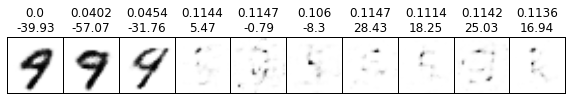
\includegraphics[width=0.4\textwidth]{gen}}
	\subfigure[weight]{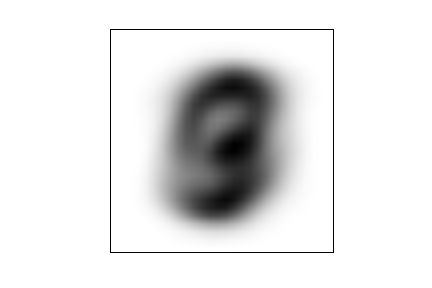
\includegraphics[width=0.4\textwidth]{weights}}
	\subfigure[inverted weight]{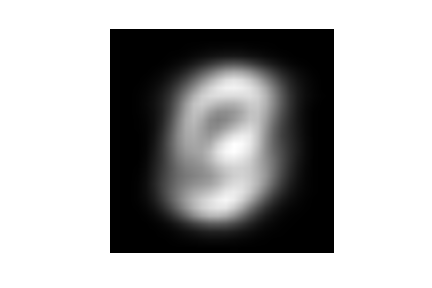
\includegraphics[width=0.4\textwidth]{inv_weights}}
	\subfigure[weighted corrupted digit]{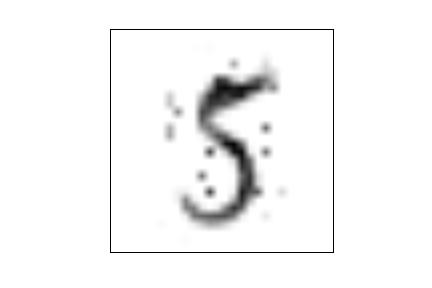
\includegraphics[width=0.4\textwidth]{nw}}
	\subfigure[weighted generated digit]{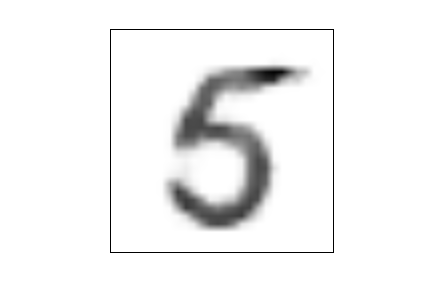
\includegraphics[width=0.4\textwidth]{gw}}
	\centering
	\subfigure[mixed digit]{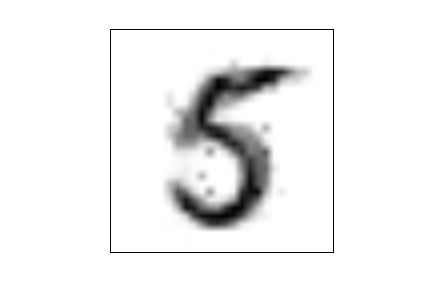
\includegraphics[width=0.4\textwidth]{mix}}
	\caption{Mixing process example}
	\label{fig:mixing}
\end{figure}

\subsection{Conclusion} % (fold)
\label{sub:conclusion}



% subsection conclusion (end)
\pagebreak
\input{../KDeepBeliefNetwork_summer/tempSummary.tex}




\bibliography{MNISTSummary}
\bibliographystyle{plain}

\end{document}

% Yann LeCun A Tutorial on Energy-Based Learning
%Hinton02: training products of experts by minimizing contrastive divergence

